\documentclass[conference]{IEEEtran}
\IEEEoverridecommandlockouts
% The preceding line is only needed to identify funding in the first footnote. If that is unneeded, please comment it .
%Template version as of 6/27/2024

\usepackage{cite}
\usepackage{amsmath,amssymb,amsfonts}
\usepackage{algorithmic}
\usepackage{graphicx}
\usepackage{textcomp}
\usepackage{xcolor}
\usepackage{subcaption}
\def\BibTeX{{\rm B\kern-.05em{\sc i\kern-.025em b}\kern-.08em
    T\kern-.1667em\lower.7ex\hbox{E}\kern-.125emX}}
\begin{document}

\title{Implementation of Binary Classification\\
%{\footnotesize \textsuperscript{*}Note: Sub-titles are not captured for https://ieeexplore.ieee.org  and
%should not be used}
%\thanks{Identify applicable funding agency here. If none, delete this.}
}

\author{\IEEEauthorblockN{Jiaqi Yin}
%\IEEEauthorblockA{\textit{dept. name of organization (of Aff.)} \\
%\textit{name of organization (of Aff.)}\\
%City, Country \\
%email address or ORCID}
%\and
%\IEEEauthorblockN{2\textsuperscript{nd} Given Name Surname}
%\IEEEauthorblockA{\textit{dept. name of organization (of Aff.)} \\
%\textit{name of organization (of Aff.)}\\
%City, Country \\
%email address or ORCIDsudo tlmgr update --self}
%\and
%\IEEEauthorblockN{3\textsuperscript{rd} Given Name Surname}
%\IEEEauthorblockA{\textit{dept. name of organization (of Aff.)} \\
%\textit{name of organization (of Aff.)}\\
%City, Country \\
%email address or ORCID}
%\and
%\IEEEauthorblockN{4\textsuperscript{th} Given Name Surname}
%\IEEEauthorblockA{\textit{dept. name of organization (of Aff.)} \\
%\textit{name of organization (of Aff.)}\\
%City, Country \\
%email address or ORCID}
%\and
%\IEEEauthorblockN{5\textsuperscript{th} Given Name Surname}
%\IEEEauthorblockA{\textit{dept. name of organization (of Aff.)} \\
%\textit{name of organization (of Aff.)}\\
%City, Country \\
%email address or ORCID}
%\and
%\IEEEauthorblockN{6\textsuperscript{th} Given Name Surname}
%\IEEEauthorblockA{\textit{dept. name of organization (of Aff.)} \\
%\textit{name of organization (of Aff.)}\\
%City, Country \\
%email address or ORCID}
}

\maketitle

%\begin{abstract}
%This document is a model and instructions for \LaTeX.
%This and the IEEEtran.cls file define the components of your paper [title, text, heads, etc.]. *CRITICAL: Do Not Use Symbols, Special Characters, Footnotes,
%or Math in Paper Title or Abstract.
%\end{abstract}

\begin{IEEEkeywords}
Classification, NLP
\end{IEEEkeywords}

\section{Introduction}
In this paper, I will implement several binary state of art classification on two types of datasets. 

\section{Dataset 1: Bank Marketing Campaign Subscription}
In the following sections, I will describe the dataset, preprocessing steps, implemented models, hyperparameter tuning, results analysis, and sensitivity analysis by feature reduction.

\subsection{Data Description}
The dataset, obtained from Kaggle \cite{b1}, contains records of marketing phone calls from a Portuguese banking institution. The calls were conducted to persuade bank customers to subscribe to a specific financial product. For each call, customers indicated their willingness to subscribe, serving as an indicator of campaign success.

This dataset is interesting for several reasons:
\begin{itemize}
    \item It presents a binary classification problem with a relatively large sample size ($N=41,188$).
    \item The data is imbalanced (yes: $11.3\%$, no: $88.7\%$).
    \item It contains both numerical and categorical features, requiring diverse preprocessing techniques.
    \item As real-world data, it has practical applications in industry.
\end{itemize}

The dataset comprises 41,188 phone call records with 20 features, covering multiple aspects of the customers, such as demographics (e.g., age, job, education), previous campaign contact and outcome, and socio-economic context. The target variable is the campaign outcome: 'yes' or 'no' to subscribing to the product.

My objective is to predict whether a customer will subscribe to the product based on the available information. I will implement several binary classification models to predict the campaign outcome and compare their performance.

\subsection{Data Preprocessing and Exploration}
Of the 20 features, 10 are numerical and 10 are categorical. The numerical feature \textit{pdays} (number of days since the client was last contacted from a previous campaign) has a value of 999 for clients not previously contacted, which constitutes the majority. Considering its importance, I converted it into a categorical variable with the following categories: \textit{NoContact, 0-2, 3-7, 8-14, $>14$}.

Numerical features contain some outliers that could distort the model, and most are skewed; see in Fig \ref{fig:features}. To improve performance, I implemented the following steps:
\begin{enumerate}
    \item Clipped outliers using the IQR method with a 2.0 threshold.
    \item Standardized numerical features using StandardScaler.
\end{enumerate}

\begin{figure}[htbp]
    \centering
    \begin{subfigure}[b]{0.45\textwidth}
        \centering
        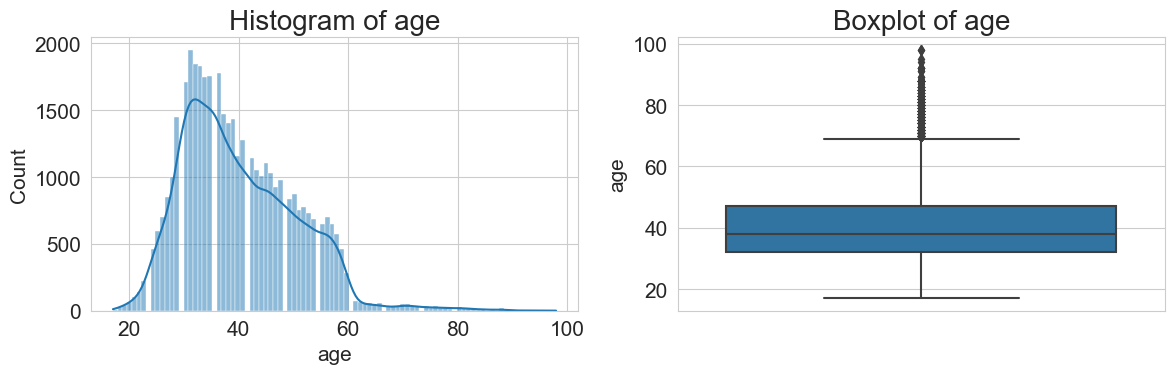
\includegraphics[width=\textwidth]{figs/age_distribution.png}
        \caption{Feature Age Distribution}
        \label{fig:feature_age}
    \end{subfigure}
    \hfill
    \begin{subfigure}[b]{0.45\textwidth}
        \centering
        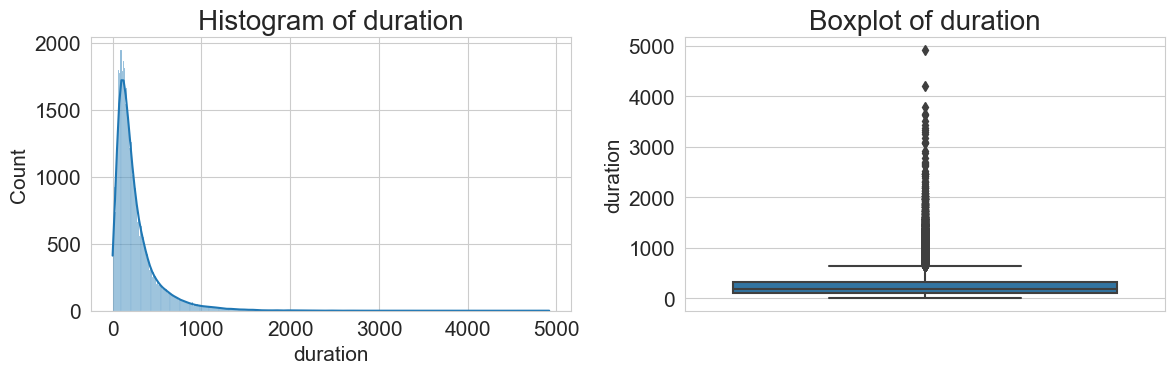
\includegraphics[width=\textwidth]{figs/duration_distribution.png}
        \caption{Feature Duration Distribution}
        \label{fig:feature_duration}
    \end{subfigure}
    \caption{Numerical feature examples with outliers and skewed distribution. Age is the client's age, and duration is the last contact duration in seconds.}
    \label{fig:features}
\end{figure}

For categorical features, I applied one-hot encoding to convert them into numerical format. 

After the feature preprocess, the dataset contains 67 features. To reduce the feature set, I implemented a feature importance analysis using the Gradient Boosting Tree model which is discussed in Section. 

For model training and testing, I split the dataset into a training set and a testing set with a 4:1 ratio. For hyperparameter tuning, I employed five-fold cross-validation on the training set.

\subsection{Model Implementation and Hyperparameter Tuning}
I implemented four models using the scikit-learn library: K-Nearest Neighbors (KNN), Support Vector Machine (SVM), Neural Network (NN), and Gradient Boosting Tree (GBT). For all models, I used 5-fold cross-validation for hyperparameter tuning. Due to limited computational resources on my local desktop, I had to balance the breadth of hyperparameter exploration with computational feasibility.

\subsubsection{KNN}
I used \verb|KNeighborsClassifier| for KNN implementation. To study the effect of the number of neighbors, I explored the range of $K = \{3, 5, 10, 15, 20, 25, 30\}$ using Euclidean distance. This range was chosen to cover both small and large neighborhood sizes without prior knowledge of the optimal value. I also explored two weight options:
\begin{itemize}
    \item Uniform: All neighbors have equal weight.
    \item Distance: Neighbors are weighted by the inverse of their distance, giving closer neighbors greater influence.
\end{itemize}

\subsubsection{SVM}
I used \verb|sklearn.svm.SVC| for SVM implementation. I explored the following hyperparameters:
\begin{itemize}
    \item Kernel: 'poly', 'rbf', 'sigmoid'
    \item $\gamma$: 'scale', 'auto', 0.1, 0.01
\end{itemize}

These kernels are widely used in practice:
\begin{itemize}
    \item Polynomial (poly): Can model non-linear relationships of higher degree.
    \item Radial Basis Function (rbf): Effective for non-linear boundaries in many cases.
    \item Sigmoid: Can produce results similar to certain neural networks.
\end{itemize}

The $\gamma$ parameter contral the spread of the influence of each point. Lower values leads to a smoother decision boundary, while higher values can lead to overfitting.

\subsubsection{NN}
I used MLPClassifier for NN implementation. With 67 total features, I explored various hidden layer configurations:
\begin{itemize}
    \item One hidden layer: 5, 10, 15, 20, 25, 30, 35, 40, 45, 50 neurons
    \item Two hidden layers: [32, 5], [32, 10], [32, 15], [32, 20], [32, 25], [32, 30], [32, 32] neurons
\end{itemize}

I used 'adam' as the optimization algorithm, 'relu' activation for hidden layers, and 'sigmoid' activation for the output layer. The initial configuration used a constant learning rate of 0.001, batch size of 200, and maximum of 200 epochs. To prevent overfitting, I employed early stopping.

Given the importance of learning rate in neural network training, I further explored adaptive learning rates with different initial values: 1.0, 0.5, 0.1, 0.08, 0.06, 0.04, 0.02, 0.01, 0.005, 0.001, 0.0005, 0.0001.

\subsubsection{GBT}
I used \verb|GradientBoostingClassifier| for GBT implementation. I explored the following hyperparameters:
\begin{itemize}
    \item Number of estimators (boosting stages): 50, 100, 150, 200
    \item Maximum tree depth: 3, 5, 7, 9
    \item Subsample ratio: 0.5, 0.7, 0.9, 1.0
\end{itemize}

These hyperparameters were tuned to balance model complexity and performance. The number of estimators and max depth affect the model's capacity to learn complex patterns, while the subsample ratio helps in reducing overfitting by introducing randomness in the training process.

I also leveraged the feature importance from GBT to perform feature reduction, which will be discussed in a later section. This approach capitalizes on the boosting tree's ability to learn which combination of features significantly reduces the fitting error.

\subsection{Results and Analysis}


\begin{table}[htbp]
\caption{Table Type Styles}
\begin{center}
\begin{tabular}{|c|c|c|c|}
\hline
\textbf{Table}&\multicolumn{3}{|c|}{\textbf{Table Column Head}} \\
\cline{2-4} 
\textbf{Head} & \textbf{\textit{Table column subhead}}& \textbf{\textit{Subhead}}& \textbf{\textit{Subhead}} \\
\hline
copy& More table copy$^{\mathrm{a}}$& &  \\
\hline
\multicolumn{4}{l}{$^{\mathrm{a}}$Sample of a Table footnote.}
\end{tabular}
\label{tab1}
\end{center}
\end{table}

% \begin{figure}[htbp]
% \centerline{\includegraphics{fig1.png}}
% \caption{Example of a figure caption.}
% \label{fig}
% \end{figure}



\begin{thebibliography}{00}
\bibitem{b1} Bank Marketing Campaign Subscription data source: https://www.kaggle.com/datasets/pankajbhowmik/bank-marketing-campaign-subscriptions

\end{thebibliography}

\vspace{12pt}
\color{red}
IEEE conference templates contain guidance text for composing and formatting conference papers. Please ensure that all template text is removed from your conference paper prior to submission to the conference. Failure to remove the template text from your paper may result in your paper not being published.

\end{document}
